

\documentclass[compress]{beamer}

\usepackage{thumbpdf}
\usepackage{wasysym}
\usepackage{ucs}
\usepackage[utf8]{inputenc}
\usepackage{pgf,pgfarrows,pgfnodes,pgfautomata,pgfheaps,pgfshade}
\usepackage{pgfpages}
\usepackage{verbatim}
\usepackage{fancyvrb}
\usepackage{multimedia}
\usepackage{subcaption}
\usepackage{ulem}
\usepackage{textcomp}
\usepackage{tikz}

\usepackage{listings}

\usepackage{epigraph}
\setlength{\epigraphwidth}{.8\textwidth}

\usepackage{DejaVuSansMono}

\usepackage{multicol}  
\usepackage{media9}

% Adjust the colours to fit your design
\definecolor{mainthemecolour}{rgb}{0.42,0.48,0.37}
\definecolor{mainthemecolourlight}{rgb}{0.63,0.72,0.57}
\definecolor{mainthemecolourstrong}{rgb}{0.40,0.68,0.18}
\definecolor{mid-gray}{gray}{0.7}

\definecolor{greenstrong}{rgb}{0.58,0.77,0.29}
\definecolor{redstrong}{rgb}{0.81,0.22,0.23}
\definecolor{fglisting}{gray}{0.3}
\definecolor{bglisting}{gray}{1}
\definecolor{fgshell}{gray}{1}
\definecolor{bgshell}{gray}{0.1}
\definecolor{bgshelllight}{gray}{0.8}


% Some in-code macros - a bit buggy, but useful
\newcommand{\hl}[1]{\textcolor{greenstrong}{\texttt{#1}}}
\newcommand{\hlErr}[1]{\textcolor{redstrong}{\texttt{#1}}}
\newcommand{\hlOk}[1]{\textcolor{green}{\texttt{#1}}}
\newcommand{\hlInv}[1]{\colorbox{bgshell}{\textcolor{fgshell}{\texttt{#1}}}}

\newcommand{\unhl}[1]{\textcolor{gray}{#1}}
\newcommand{\clda}[0]{$\textcolor{blue}{\lambda}$}
\newcommand{\carr}[0]{$\textcolor{purple}{\rightarrow}$}
\newcommand{\cbind}[0]{\textbf{\texttt{$>\!\!>\!\!=$}}}
\newcommand{\codedots}[0]{\textcolor{mid-gray}{...}}

\usetheme{elegance}

\lstnewenvironment{cxxcode}
    {\lstset
        { escapeinside={@}{@}
        , gobble=8
        , showstringspaces=false
        , basicstyle=\color{fglisting}
        , rulecolor=\color{mainthemecolourlight}
        }
    }
    {}

\lstnewenvironment{cxxcodebox}
    {\lstset
        { escapeinside={@}{@}
        , gobble=6
        , showstringspaces=false
        , basicstyle=\color{fglisting}
        , frame=lr
        , rulecolor=\color{mainthemecolourlight}
        }
    }
    {}

\lstnewenvironment{shellcode}
    {\lstset
        { escapeinside={@}{@}
        , gobble=7
        , showstringspaces=false
        , basicstyle=\color{fgshell}
        , backgroundcolor=\color{bgshell}
        }
    }
    {}


% Marking points to use in Tikz
\usetikzlibrary{arrows,shapes}
\newcommand{\tikzmark}[1]{\tikz[remember picture] \node[coordinate] (#1) {#1};}

% Fragile frames
\newenvironment{xframe}[1][]
  {\begin{frame}[fragile,environment=xframe,#1]}
  {\end{frame}}



\title{\hei{时间序列数据驱动下的深度学习模型研究}}
\subtitle{个人简介与研究课题论证}
\author{张心泽}

\institute{\color{white}
    xinze@hust.edu.cn \\
    https://github.com/XinzeZhang
} %
\date{\footnotesize\color{mainthemecolour} HUST, Wuhan 2018. }



\begin{document}
\hypersetup{pdfpagemode=FullScreen}
\maketitle
\section{个人简介}

\subsection{教育背景}

\begin{xframe}{\kai{教育背景}}
    \cveducation
    {\entrylocationstyle{华中科技大学}}
    { }

    \vspace{2.0mm}

    \cvsubeducation
    {计算机科学与技术学院}
    {09/2016 - 02/2017}

    \vspace{-2.5mm}
    \begin{itemize}
        \item \descriptionstyle{计算机科学与技术,选修,GPA:3.6/4.0}
        \item \descriptionstyle{\itshape{核心课程: 高等工程数学(矩阵论 \& 数理统计 \& 数值计算), 人工智能, 模式识别, 知识发现与数据开采, 大数据技术, 启发式优化}}
    \end{itemize}

    \cvsubeducation
    {管理学院}
    {09/2015 - 06/2016}

    \vspace{-2.5mm}
    \begin{itemize}
        \item \descriptionstyle{会计硕士,主修, GPA 3.8/4.0}
        \item \descriptionstyle{\itshape{核心课程: 财务管理理论与实务, 管理会计理论与实务, 审计理论与实务,内部控制理论与实务,金融市场与金融工具}}
    \end{itemize}

\end{xframe}

\begin{xframe}{\kai{教育背景}}
    \cveducation
    {\entrylocationstyle{中南财经政法大学}}
    { }

    \vspace{2.0mm}

    \cvsubeducation
    {会计学院}
    {09/2011 - 06/2015}

    \vspace{-2.5mm}

    \begin{itemize}
        \item \descriptionstyle{会计学学士}
        \item \descriptionstyle{\itshape{核心课程: 会计学原理,中级会计学,管理会计学(双语),企业资源计划,会计实验学,会计电算化}}
    \end{itemize}

\end{xframe}

\subsection{研究经历}

\begin{xframe}{\kai{研究经历}}
    \cvexperience
    {\entrylocationstyle{研究助理},蔡淑琴教授,管理学院}
    {09/2015 - 08/2017}

    \vspace{-2.5mm}

    \begin{itemize}
        \item \descriptionstyle{结合句法结构与向量空间模型,提出一种考虑抱怨问题路径的网络抱怨识别方法;}
        \item \descriptionstyle{考虑知识、情感和互动三个资源维度,建立处理在线负面口碑的专家识别方法;}
        \item \descriptionstyle{参与大数据实验室的建设,撰写17年国家自科基金项目申请书中关于大数据产品质量测度的部分;}
    \end{itemize}

    \cvexperience
    {\entrylocationstyle{研究助理},大数据实验室,管理学院}
    {03/2016 - 08/2017}

    \vspace{-2.5mm}

    \begin{itemize}
        \item \descriptionstyle{利用有源标签信号强度在多个接收器的差别,实现基于ZigBee的区域定位接口;}
        \item \descriptionstyle{搭建基于Hadoop的全分布式计算机集群,实现Map/Reduce框架下的Naïve Bayes分类器;}
    \end{itemize}

\end{xframe}

\begin{xframe}{\kai{研究经历}}
    \cvexperience
    {\entrylocationstyle{研究实习},何琨教授,计算机学院}
    {07/2017 - PRESENT}

    \vspace{-2.5mm}

    \begin{itemize}
        \item \descriptionstyle{提出会计事项的机器理解方法,利用Word2Vec方法实现会计事项的词向量空间嵌入;}
        \item \descriptionstyle{提出会计分录的机器编制方法,利用GRUs+Attention机制实现会计知识的深度学习;}
        \item \descriptionstyle{探索神经网络的随机逼近方法,利用随机权重机制进行神经网络参数的快速寻优;}
        \item \descriptionstyle{探索深度神经网络的解释性,尝试利用随机权重机制解释神经网络的训练过程;}
    \end{itemize}
\end{xframe}

\subsection{教学经历}

\begin{xframe}{\kai{教学经历}}
    \cvexperience
    {\entrylocationstyle{助理教师},蔡淑琴教授,管理学院}
    {03/2016 - 09/2017}

    \vspace{-2.5mm}

    \begin{itemize}
        \item \descriptionstyle{MBA课程:电子商务}
        \item \descriptionstyle{本科生课程:管理信息系统分析与设计,专业概论,课程设计,生产实习(信息管理与信息系统)}
    \end{itemize}

    \vspace{1.0mm}
    \cvexperience
    {\entrylocationstyle{助理教师},石双元教授,管理学院}
    {09/2016 - 01/2017}

    \vspace{-2.5mm}

    \begin{itemize}
        \item \descriptionstyle{本科生课程:信息系统开发方法与工具(C\#)}
    \end{itemize}

    \vspace{1.0mm}
    \cvexperience
    {\entrylocationstyle{助理教师},张千帆教授,管理学院}
    {09/2015 - 01/2016}

    \vspace{-2.5mm}

    \begin{itemize}
        \item \descriptionstyle{本科生课程:数据结构(C/C++),数据库技术及应用}
    \end{itemize}
\end{xframe}

\subsection{工程经历}

\begin{xframe}{\kai{工程经历}}
    \cvexperience
    {\entrylocationstyle{系统工程师},华威科智能股份有限公司}
    {11/2016 - 08/2017}

    \vspace{-2.5mm}

    \begin{itemize}
        \item \descriptionstyle{主导设计并参与开发一套武术体育竞赛管理信息系统;}
        \item \descriptionstyle{负责整套系统的需求分析、信息模型设计、功能设计、数据库设计和功能测试等;}
        \item \descriptionstyle{独立负责运动员管理与检录的开发工作,基于RFID实现运动员自动化注册和检录;}
        \item \descriptionstyle{承担2016年湖南省武术比赛、2017年湖北省青少年武术锦标赛的竞赛管理;}
    \end{itemize}

    \cvexperience
    {\entrylocationstyle{程序员},管理学院MPACC中心}
    {03/2018}

    \vspace{-2.5mm}

    \begin{itemize}
        \item \descriptionstyle{设计并基于RFID开发一套研究生复试检录抽签系统;}
    \end{itemize}

\end{xframe}

{
\usebackgroundtemplate{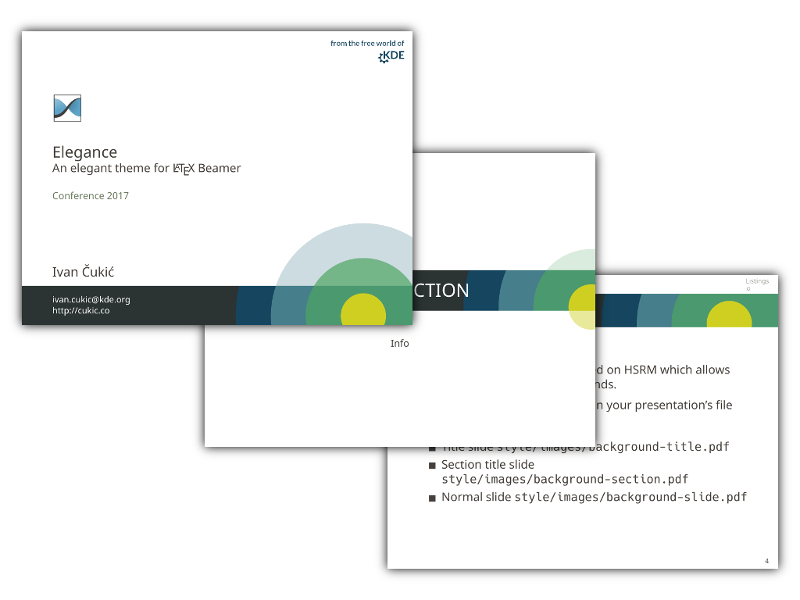
\includegraphics[width=\paperwidth]{../screenshots/theme-1.png}}
\begin{frame}[plain]
    .
\end{frame}
}


{
\usebackgroundtemplate{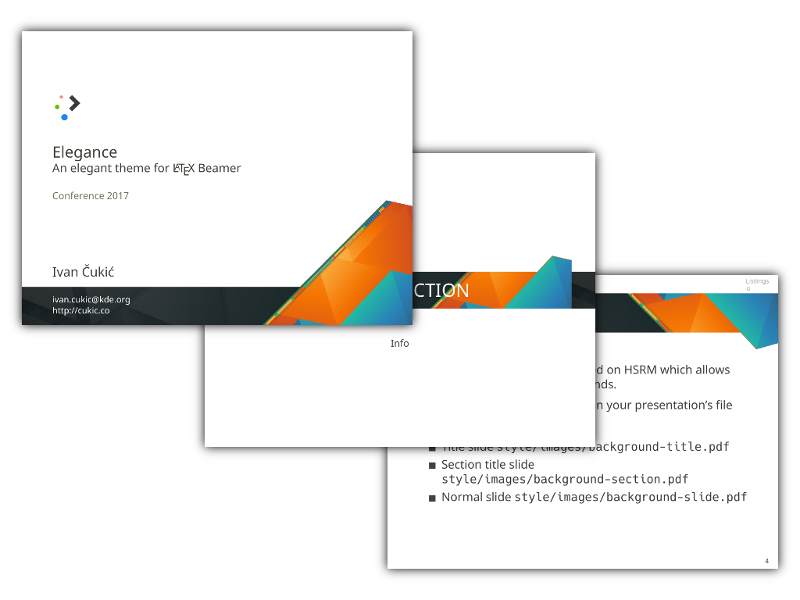
\includegraphics[width=\paperwidth]{../screenshots/theme-2.png}}
\begin{frame}[plain]
    .
\end{frame}
}


{
\usebackgroundtemplate{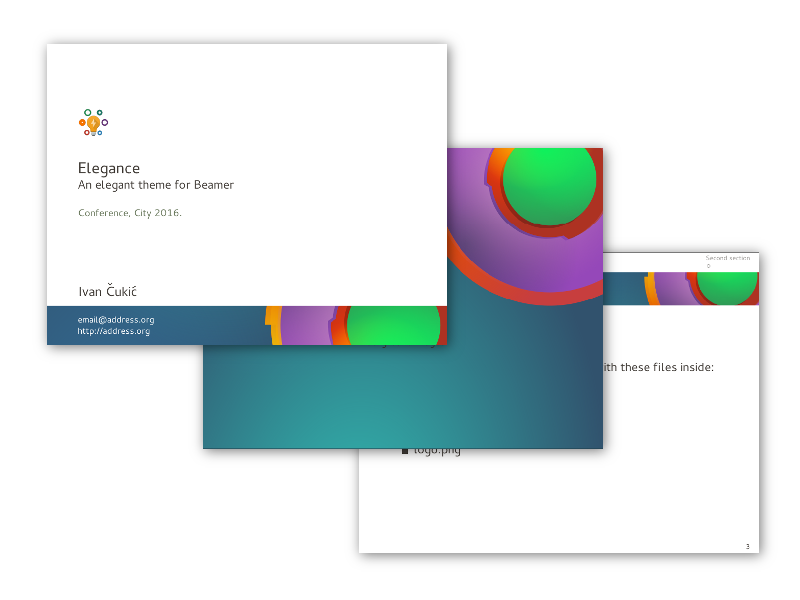
\includegraphics[width=\paperwidth]{../screenshots/theme-3.png}}
\begin{frame}[plain]
    .
\end{frame}
}





\section{Examples}

\subsection{Showing code}

\begin{xframe}{Code snippets}

    Do you have some code to show on the slide?

    And the same frame should also contain text?

    \begin{cxxcodebox}
        class example {
                // \codedots shows grayed-out dots
                @ \codedots @
            };
    \end{cxxcodebox}

    You can use \verb|cxxcodebox| environment.
    It has \verb|cxx| in the name,
    but no syntax highlighting is performed.

    For short code snippets,
    it is better just to highlight the important parts.

\end{xframe}


\subsection{Code slides and escapes}

\begin{xframe}{Second slide}

    \begin{cxxcode}
        class example {
                // There are a few useful escapes here
                @ \codedots @ // \codedots shows grayed-out dots

                // Invalid parts can be marked with \hlErr
                @\hlErr{operator;}@

                // Good parts can be marked with \hlOk
                @\hlOk{operator() ()}@

                // Other highlighting commands can be seen in
                // the preamble.tex file
            };
    \end{cxxcode}

\end{xframe}

\end{document}
